\setcounter{chapter}{-1}
%%%%%%%%%%%%%%%%%%
\chapter{Proposal Summary}
%%%%%%%%%%%%%%%%%%

This chapter will not be part of the final thesis but serves as more of an executive summary of where I am in the thesis process.
\Cref{tab:timeline} describe the notional timeline of my doctoral work.
The following to sections briefly summarize the papers I have completed so far, and the papers that I plan to publish to complete my thesis.
More substantial descriptions of the work are given in the body of thesis.


\begin{table}
  \centering
  \begin{tabular}{lll}
  \toprule
  2019 & August & Began research master's degree (CMU) \\
  2021 & August & Completed masters, began PhD \\
  2024 & July--September & XferBench eval (\Cref{ch:xferbench-analysis}) \\
  & September & Proposal \\
  & October--December & Rich corpora (\Cref{ch:rich-corpora}) \\
  2025 & January--March & Morphemes (\Cref{ch:morphemes}) \\
  & April--June & Morpheme structure (\Cref{ch:syntax}) \\
  & July & Defense \\
  \bottomrule
  \end{tabular}

  \caption{Timeline}
  \unskip\label{tab:timeline}
\end{table}

\section{Completed Work}
% The following completed research papers will be incorporated into the thesis (either in part or their entirety).
% Other work has be published and/or completed during the course of my master's and doctoral work but will not play major role in the thesis.


\subsection{Recommendations for Systematic Research on Emergent Language}
\noindent
\citet{boldt2022recommendations} was rejected from ICML 2022; part of this work was expanded into ``A Review of the Applications of Deep Learning-Based Emergent Communication'' discussed below.
This is a position paper which critiques and makes recommendations for emergent communication research from a meta-scientific angle.
It begins by specifying the goals of emergent communication research (which would eventually become the TMLR paper).
In light of these goals, which are split between ``engineering'' and ``scientific'' goals, the paper discusses core methodological elements of engineering and science.
Finally, each of the core methodological elements is explicitly detailed in the context of emergent communication.
In addition to the goals, the particular elements of engineering which are pursued in this thesis are evaluation metrics and standard datasets.

\subsection{A Review of the Applications of Deep Learning-Based Emergent Communication}

\noindent
\citet{boldt2024review} was published in the \textit{Transactions of Machine Learning Research} (TMLR) in February 2024.
This paper comprehensively reviews the applications and goal of emergent communication research drawing on both the literature and the author's (i.e., Brendon and David's) experience in the field.
Each application, in addition to a description and review of the relevant literature, is a accompanied by a brief set of recommendations on the most fruitful next steps for that research direction.
The set of applications themselves is divided into three categories:
  (1) internal applications, which focus on improving the methods of emergent communication itself,
  (2) task-driven applications, which look at engineering tasks focused on more effectively solving particular problems,
  and (3) knowledge-driven applications, which aim at increasing scientific understanding of particular phenomena.

\subsection{XferBench: a Data-Driven Benchmark for Emergent Language}
\noindent
\citet{boldt2024xferbench} was published in the \textit{Proceedings of the 2024 Conference of the North American Chapter of the Association for Computational Linguistics: Human Language Technologies (Volume 1: Long Papers)} (NAACL).
This paper introduces a first-of-its-kind evaluation metric/benchmark for emergent languages.
It addresses the question of the \emph{quality} of an emergent language by looking at its similarity to human language from a data-driven, machine learning perspective.
Specifically, it quantifies ``similarity to human language''---and, therefore, overall quality---as how much pretraining on an emergent language corpus improves performance on modeling human language (although we also test machine translation).
XferBench is published as an easy-to-use Python package, and since it only requires an unannotated corpus of utterances from the emergent language, it is intended to have widespread use in emergent communication research.


\subsection{ELCC: the Emergent Language Corpus Collection}
Under review at the \textit{2024 Conference on Neural Information Processing Systems Datasets and Benchmarks Track} (decision in September 2024).
This paper introduces a collection of over $70$ emergent language corpora from across $8$ different systems in the literature.
Each of these corpora is annotated with statistical analyses as well as metadata documenting the features of the system/environment it came from.
Such a resource is intended to make studying emergent languages themselves far easier since it obviates the need run the systems oneself and enable comparative studies given the variety of emergent communication systems included.

\subsection{Other Work}
Some work completed during the course of master's and doctoral work will not factor heavily into the thesis.
In ``Mathematically modelling the lexicon entropy of emergent language'' \citep{boldt2022mathematically}, we investigate using a formal model based on the Chinese restaurant process to make predictions of the entropy of lexica in emergent languages; this is intended to be a sort of exemplar of using formal models to make clear, determinate hypotheses regarding emergent communication experiments.
In ``Shaped rewards bias emergent language'' \citep{boldt2022shaped}, we argue that reward shaping (a common feature of reinforcement learning experiments) has the potential to bias (i.e., predetermine) properties of the resulting emergent language.
In ``Case study: deontological ethics in NLP'' \citep{prabhumoye-etal-2021-case}, we apply deontological approach to ethics to different real-world scenarios in natural language processing-based systems.



\section{Proposed Work}
This section will briefly described the proposed work for the completion of the doctoral thesis.
Each of these papers is intended to a standard conference-length paper (i.e., 8--9 pages).

\subsection{XferBench analysis}
In this paper, which is currently in progress, we will run XferBench on all of the languages in ELCC in order to find correlations between XferBench performance and features of the corpora and emergent communication system they come from.
For example, we hope to answer question such as ``Do more complex environments yield better emergent languages?'' or ``Is token entropy of an emergent language predictive of its score on XferBench?''
These analyses will help to understand what XferBench is measuring and whether it is easily explainable by surface-level statistics of the corpus or whether some deeper structural characteristics might be required to understand XferBench's outputs.


\subsection{Rich emergent language corpora}
ELCC, the current collection of emergent language corpora, only includes the corpora themselves and aggregate statistics, but many interesting research directions require not only having access to the tokens of utterances themselves but also their context.
For example, anything related to semantics is going to require some way to determine what an utterance means.
Thus, we propose an extension to ELCC which takes the same set of corpora and includes information about the state of the environment before and after each utterance so as to supply grounding for each of the utterances.
From here, it will be possible to explore a far greater range of phenomena with respect to the emergent language corpora in ELCC\@.

\subsection{Detecting linguistic universals in emergent communication}
\cmt{Edit as needed.}
This project will be the linguistic counterpart to XferBench (or at least the foundation thereof).
Whereas XferBench looks at the question of emergent language quality and similarity to human language from a data-driven, machine learning perspective, this paper will explore an evaluation metric from similarity to human language which focuses on the encoding linguistic knowledge into a detection algorithm for human language universals in emergent language corpora.
The main challenge of this paper is that many of what might be considered linguistic universals in human language already presuppose a large amount of structure within languages (e.g., morphemes), but it is has not be determined yet whether emergent languages possess anything like morphemes in human language.
Thus, before we even begin to talk about matters of syntax, it is critical to establish what morphemes look like emergent language and how to find them.
In light of this, I foresee this project focusing detecting the presence of morphemes (in some recognizable form) in emergent languages and potentially some very minimal notion of syntax built on top of any morphemes that may be present.


\subsection{Meta\"analysis of linguistic and machine learning metrics}
\cmt{Edit as needed.}
This paper is intended to be a sort of capstone of the thesis.
In short, it will determine the relationship between data-driven and linguistics-driven evaluation metrics of human language?
Is it the case that emergent languages which are better for pretraining neural models are also the ones that possess are more significant structural similarity to human languages (in linguistic terms)?
If not, is there something about the metrics that is deficient, or is perhaps the case that the linguistic and data-driven dimensions are to some extent orthogonal?
In addition to this questions, we will also explore what these metrics might tell us about creating the optimal emergent communication system that jointly maximizes all of the aforementioned metrics.




%%%%%%%%%%%%%%%%%%%%%%
\chapter{Introduction}
%%%%%%%%%%%%%%%%%%%%%%

Modern-day large language model-based AI systems are good a mimicking human language.
Some might even say they are good at \emph{using} human language, but this either imprecise or inaccurate:
  \cmt{why}.

\cmt{emergent communication a solution}

\cmt{EC is not in a great place}

\section{Background}

Emergent communication (also known as ``emergent language'') is the area of research which studies systems of communication between virtual agents that has emerged \emph{de novo} from interactions and optimizations (in the machine learning sense) in simulated environments.
Interest in this field from a deep learning perspective---which this thesis focuses on, although not exclusively---appeared in 2016 and 2017 with \cmt{papers}, and has maintained a niche though consistent following since that time.

Going backwards in time, there are papers addressing emergent communication predating deep learning methods \cmt{examples}.
More importantly, this field is strongly rooted (conceptually, though often not methodologically) in research on the origin and evolution of language in humans \cmt{citations}.

This thesis is primarily concerned with the scope of deep learning-based emergent communication.
These related fields are critical resources in developing the ideas presented hear and we hope, also, that this work will be helpful to these fields.
Nevertheless, there are many particular concerns and techniques that are unique to the deep learning-based approaches, and these are the concerns and techniques that I will primarily address.



\section{Motivation}

\cmt{discuss importance of metrics}
\cmt{emphasis of evaluation}
\cmt{discuss metrics from TMLR paper}
\cmt{why principled?}


\section{Summary of Thesis}


\subsection{Linguistic Evaluation}

\cmt{Change how this introduced to acknowledge the fact that we are not calling this ``linguistic universal detection'' anymore.}
Just as XferBench is intended to be an automatic method for determining the similarity of emergent languages to human languages according to a data-driven, deep learning approach, this chapter will introduce a method for doing the same from a linguistics-driven perspective.
Specifically, we interpret the question ``How similar is emergent language $X$ to human language generally?'' as ``To what degree does $X$ exhibit universal structural characteristics of human language?''
Some ``linguistic universals'' that come to mind 
One might immediately think of some of the universals proposed in \citet{greenberg1963universals} like ``Languages with dominant VSO order always prepositional.''
But in the case of emergent communication how can we talk about verb--subject--object ordering or prepositions when we do not even know if parts of speech properly exist---or even words for that matter?
Thus, while linguistic universals which deal with higher-order syntactic structure may be interest, it is necessary to first determine whether the low level constituent features even exist in emergent languages.

\cmt{Maybe this belongs in the introduction to motivate this and the subsequent paper.}
\cmt{I think the actual introduction for this paper will need to be much more focused.}


\begin{figure}
  \centering
  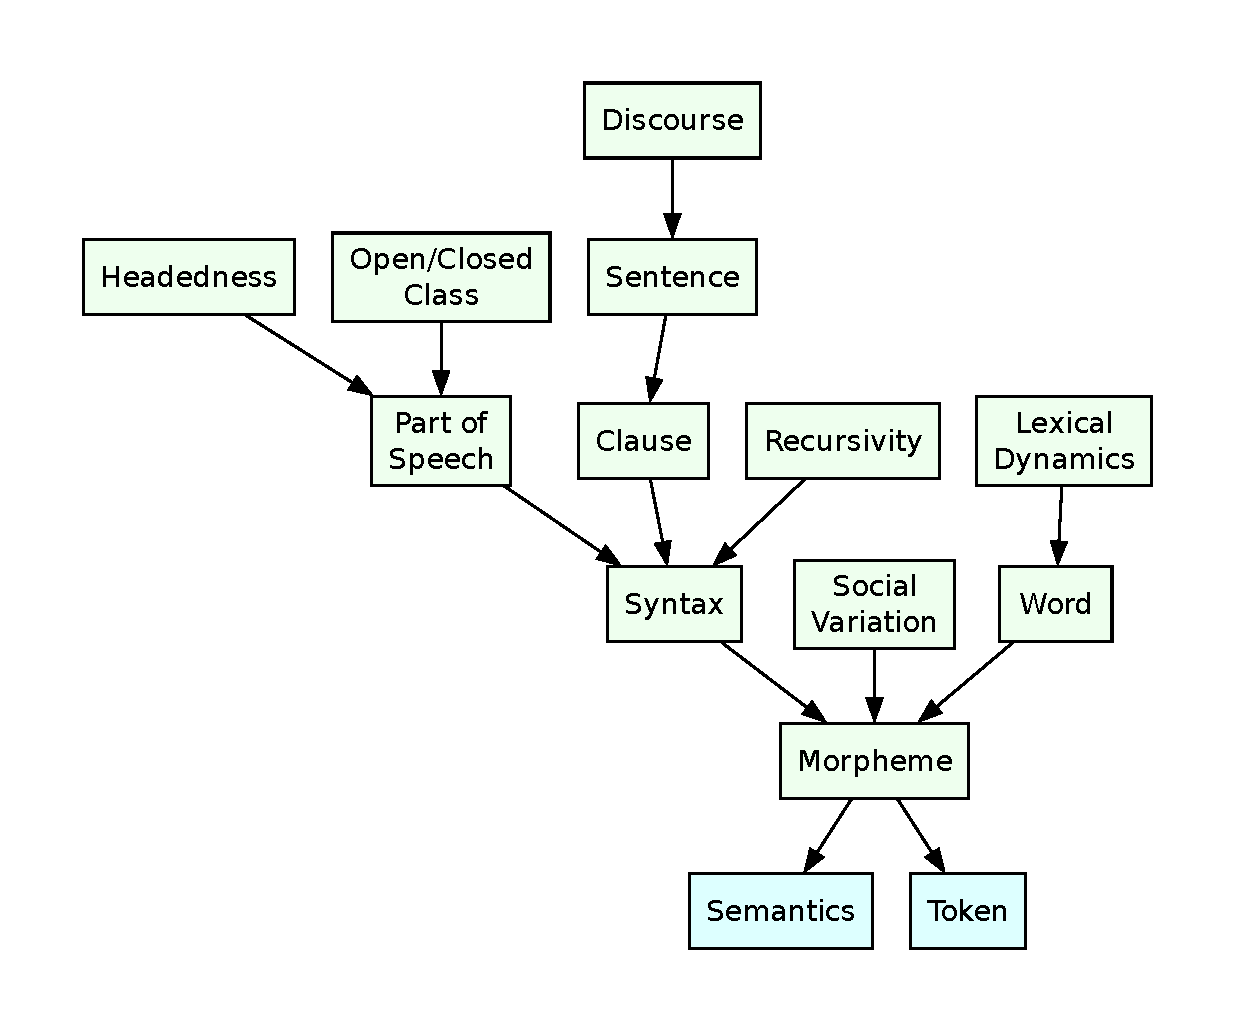
\includegraphics[width=0.95\linewidth]{assets/linguistic-dag}
  \caption{%
    Hierarchy of linguistic concepts.
    $X\rightarrow Y$ can be read as ``the definition of $X$ presupposes $Y$ being defined'' or roughly ``$X$ depends on $Y$''.
    The only concepts whose existence is established in emergent language are \emph{semantics} and \emph{token}.}
  \unskip\label{fig:linguistic-dag}
\end{figure}

In fact, there is a complex hierarchy of dependence of the various structures from across linguistics.
We illustrate hierarchy of some of the most fundamental linguistic structures in \Cref{fig:linguistic-dag}, representing the hierarchy as a transitively reduced directed acyclic graph.
At the bottom, we have foundational concepts like \emph{token} and \emph{semantics} while at the top we have concepts like \emph{headedness} and \emph{discourse}.
In the case of emergent languages, we can be sure of the existence of \emph{semantics} and \emph{tokens} and not much else.
Looking at the hierarchy, then, it would be necessary to establish the existence of \emph{morphemes} before being able to investigate phenomena like \emph{syntax} or \emph{parts of speech} in emergent communication.

\cmt{Necessary to establish the existence of, identify, define (specify, distinguish these).}

\cmt{Justify why we focus on structural characteristics?}


% \cmt{%
% Let's assume for a minute that one of the universals that we will need to detect is syntax.
% What we will need to do is create a definition of syntax in some generative sense: a language has syntax if its strings can be generated by such and such a process.
% (Is there are a more ``discriminative'' take on this process?)
% We'll need this generative take because we'll need to generate synthetic data that we can test our ``discriminative'' algorithm on given only surface forms (or surface forms + semantics).
% In addition to this generative definition, we'll need to introduce ideas of fuzziness either through non-strict adherence to the rules or by rules which inherently have some fuzz in them.
% Thus, we will have a definition of syntax which is applicable to EL since it doesn't make structural assumptions about human language as well as a process to generate synthetic data with varying levels/complexities/adherences to syntax which can for the basis of our detection algorithm.
% The idea here is that these synthetic languages will---by definition---show the full range of grammars (not necessarily very possible grammar).
% On the one hand, this feels like a bad approach because of course we can't cover every sense of grammar, but it seems like the most rigorous we can get.
% Maybe instead of saying ``we're testing for syntax full-stop'' we can say we are testing for ``$\alpha$-syntax'' which we define as being such and such: it isn't fully syntax but it is a reduced version that is easier to get to, setting a lower bar for emergent languages.
% \unskip}

Thus, this chapter will introduce an automated method for determining the presence and nature of morphemes in emergent language.
Additionally, it will also introduce a minimal definition of a syntax as proof-of-concept for identifying higher-level structures in emergent language.
These two concepts/structures are fundamental to defining and identifying other interesting features about language and so are prime candidates for foundational work in this research program.
In particular, this chapter will contribute the following items:
\begin{enumerate}[nosep]
  \item A definition of what morphemes are in the emergent languages, if they exist at all.
  \item An algorithm for determining the presence and identify of morphemes according to this definition.
  \item A minimal definition and extraction algorithm of syntax as a proof-of-concept extension of morpheme detection.
\end{enumerate}


\paragraph{Related Work}


\paragraph{Linguistics}
\cmt{URIEL \& lang2vec.}
\cmt{Compare and contrast with the ``typical'' universals which don't apply to what we have at all.}

Based on Greenberg (the whole book), there are many different kinds of universals about human language, including ones concerning:
\begin{itemize}[nosep]
  \item Presence of structures, simpliciter (the kind this chapter focuses on)
  \item Particular syntactic features; e.g., VSO \textrightarrow{} prepositional
  \item ``Design features'' of language; e.g., displaced, learnable, generalizable, evanescent
  \item Diachronic phenomena
  \item Semantics
  \item Psycholinguistics
  \item Phonology
\end{itemize}



\paragraph{Emergent communication}

\cmt{HAS paper}
\cmt{grammar induction}
\cmt{categorial grammar for compositionality}



